\documentclass[12pt]{article}
%	options include 12pt or 11pt or 10pt
%	classes include article, report, book, letter, thesis
\usepackage{amsmath,amsfonts,amssymb}
\usepackage{graphicx}
\usepackage{lipsum}
\usepackage{mwe}
\usepackage{float}
\newcommand\tab[1][1cm]{\hspace*{#1}}
\graphicspath{ {images/} }
\usepackage{hyperref}
\hypersetup{
    colorlinks=true,
    linkcolor=blue,
    filecolor=magenta,      
    urlcolor=cyan,
}

\urlstyle{same}
\begin{document}

\begin{titlepage}
\title{{\Huge Mining Uber Dataset}}
\author{Abhilash Mysore Somashekar \\Raviraj Prakash Wani \\Sanil Jain \\ Satya Akhil Chowdary Kuchipudi }
\maketitle
\end{titlepage}

\paragraph{1.	Introduction} ~\\

Uber is a smartphone-app which provides on demand ride service connecting users who need to get somewhere with drivers willing to give them a ride. The service has been hugely controversial, due to regular taxi drivers claiming that it is destroying their livelihoods, and concerns over the lack of regulatitudeion of the company's drivers, surge pricing etc. \\

The business is rooted firmly in Big Data and leveraging this data in a more effective way than traditional taxi firms have managed has played a huge part in its success. Uber's entire business model is based on the very Big Data principle of crowd sourcing. Anyone with a car who is willing to help someone get to where they want to go can offer to help get them there. \\

FiveThirtyEight obtained the data from the�NYC Limo and Taxi commission by submitting a Freedom of Information Law request on July 20, 2015. The dataset is contains on over 4.5 million Uber pickups in New York City from April to September 2014. This data was used for four FiveThirtyEight stories: Uber Is Serving New York's Outer Boroughs More Than Taxis Are, Public Transit Should Be Uber's New Best Friend, Uber Is Taking Millions Of Manhattan Rides Away From Taxis, and Is Uber Making NYC Rush-Hour Traffic Worse \\

We are extending current analysis using best practices in Data Mining to answer questions like how many pick-ups can we expect on a day, given time and at a location in NYC. We would analyze 'Hot-Spots', which are best places for drives to be to get the most pickups during a day. We would be performing Density Estimation, Gaussian Process Regression and also predict general ride patterns.  We would also study correlatitudeion between weather changes and number of Uber pickups. We would use Random Forest Regressor for predicting the number of pickups. Various data visualization techniques will be used for effective analysis of trends.

\break

\paragraph{2.	Exploratory Analysis}
\paragraph{2.1 Goals} ~\\
\begin{itemize}
	\item Preprocessing of data (rounding of the latitude and longitudes)
	\item To find out whether 4.5 million data points over 6 months are continuous or not
	\item To plot counts in histograms as well as plot Uber pickups on actual map and look at the coverage of NYC
	\item Analyze Uber pickup data over various months
	\item Finding the hotspot locations in the data. These are the locations where there are pickups more than a specified threshold
\end{itemize}

\paragraph{2.2	Graphical Analysis:} ~\\

\tab Average Pickups by Day : Comparable bars over all days of a month suggest that Uber data is continuous over the data set. Also similar graphs have been observed for rest of the months.\\
\begin{center}
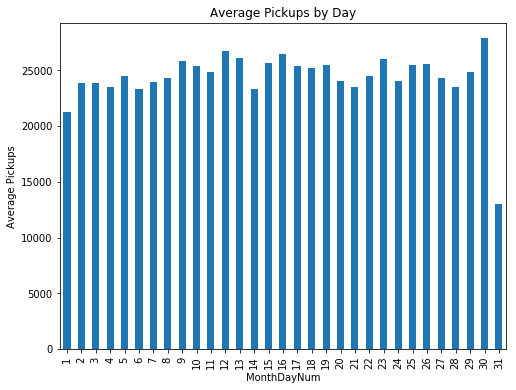
\includegraphics[width=8cm, height=7cm]{ByDay.png} 
\end{center}
\tab Average Pickups by Hour : This graph is an average of all the days data over 6 months. This suggest the evening 5:00 pm are the peak hours for Uber.\\
\begin{center}
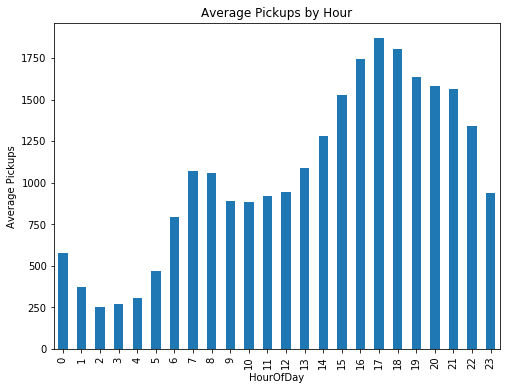
\includegraphics[width=8cm, height=7cm]{ByHour.png} 
\end{center}
\tab Average Pickups by Month (April to September) : The plot of cumulative pickups suggest that Uber business has grown over these set of months since average number of pickups have almost doubled from April to September\\
\begin{center}
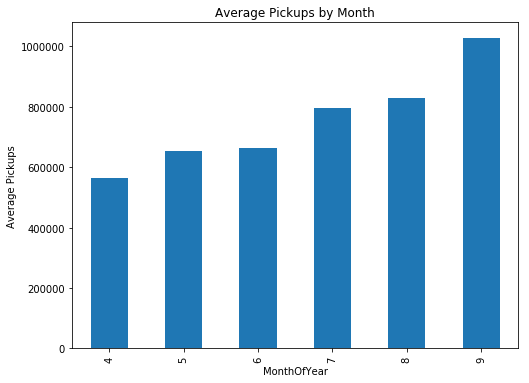
\includegraphics[width=8cm, height=7cm]{ByMonth.png}
\end{center}

\paragraph{2.3 Geographical Plot (Density Plot):}  ~\\

The complete density plot carves out the map of New York City on a black canvas by geography. This further strengthens the range of geographical data in dataset.
\begin{center}
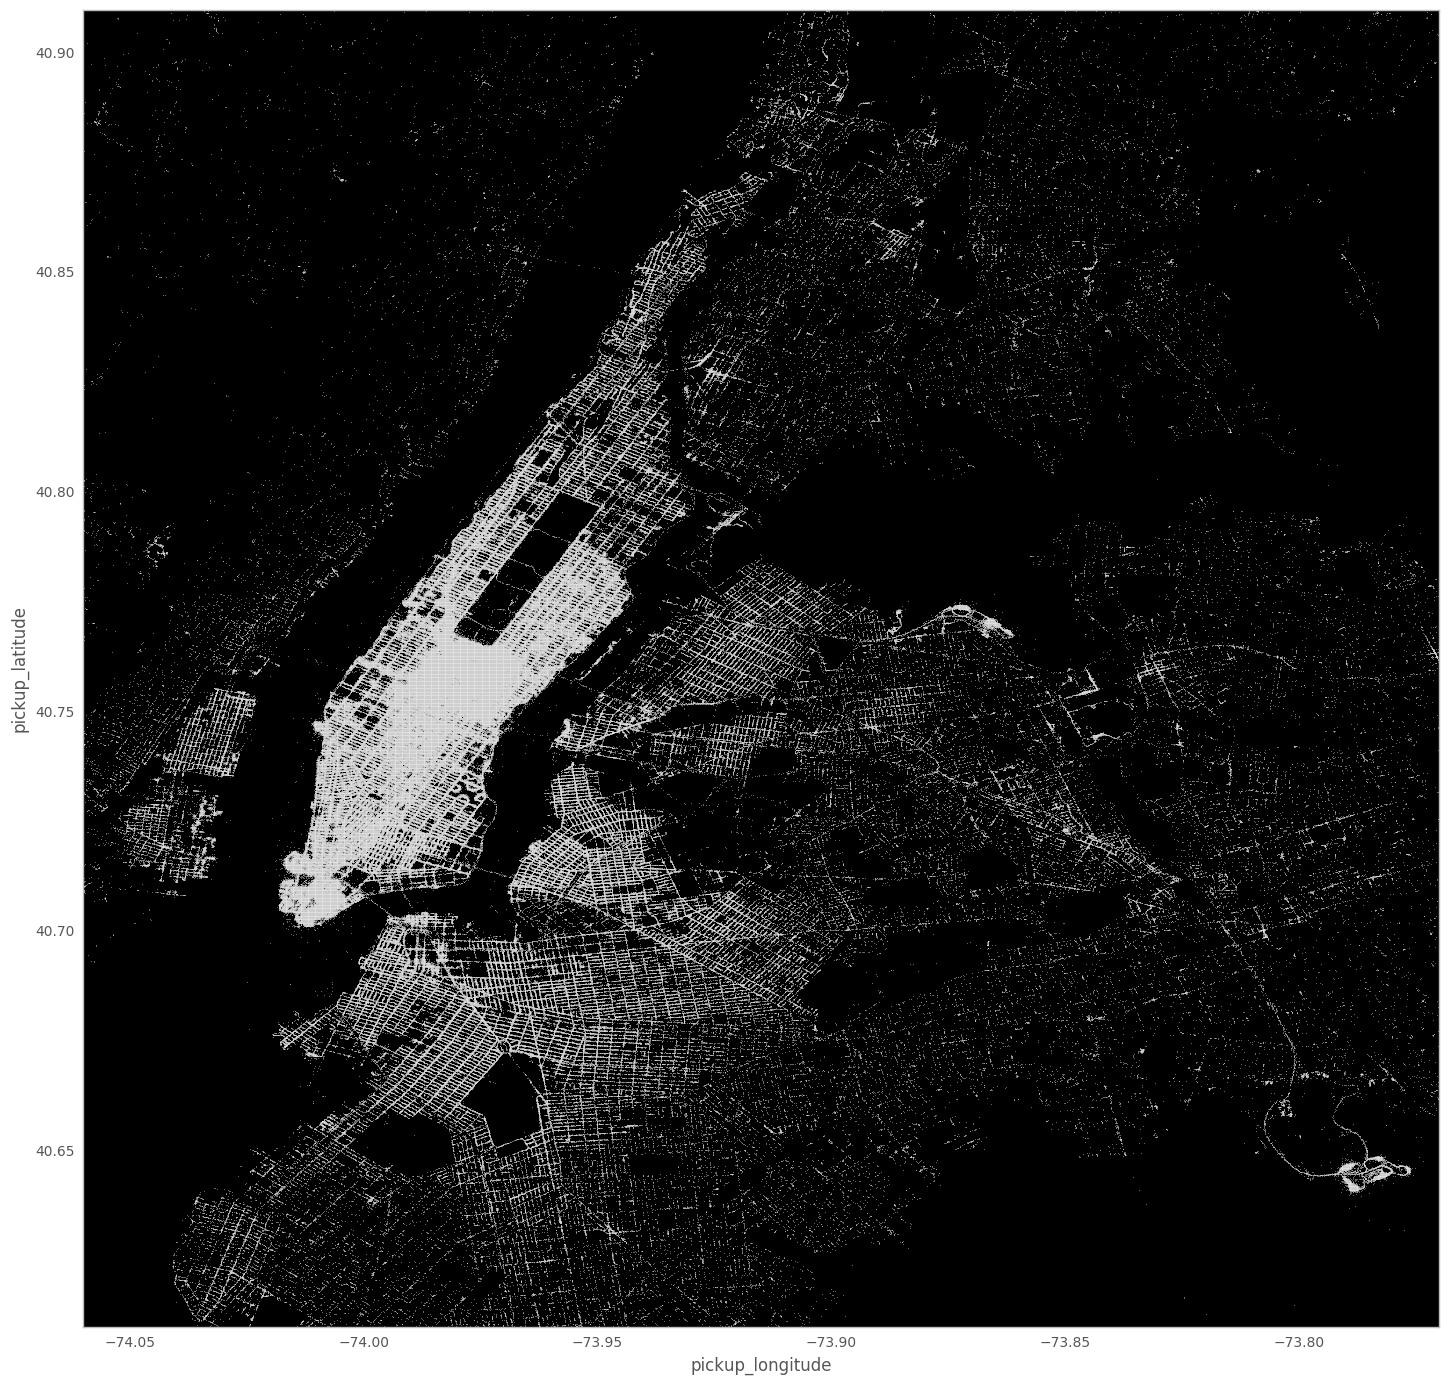
\includegraphics[width=8cm, height=8cm]{Complete.png}
\end{center}

\break

\paragraph{3  Binning and Data Reduction} ~\\

The uber-dataset for all the 6 months contains around 4.5 millions records. Binning helps in reducing the number of the input required for model creation. Also it helped us in deciding the labels required for regression. 
Binning was done based on following criterias.
\begin{itemize}
\item Time based binning : All the pickup rides are divided into 24 hours slot as per pickup time.
\item Location based binning : Entire NYC areas was divided into 'n' clusters. We used spatial DBSCAN for finding this each area center point.
\end{itemize}

\paragraph{3.1 Location based binning}~\\

Initially, we wanted to do binning for latitude-longitude based on zipcode. So we converted each latitude-longitude point to 3-decimal precision, to reduce the file size. If we round to 3 points after decimal, we are considering all points in 100m area as a single point. There are two main issues with this approach. First being that we are losing precision by rounding off and second we can't guarantee that zipcode regions are uniformly distributed areas. \\

We need to do one main change to this before we proceed with this step. We need to convert latitude-longitude point into 3-dimensional point which represents the latitude-longitude in real world. Technically we are looking at a cube space which includes all of NYC. This approach became too much technical and complex due to conversions and re-conversions. \\

We came up with a new approach for binning, that is to do a geospatial DBSCAN. We ran a geospatial DBSCAN on the latitude-longitude points to determine clusters. We didn't use euclidean distance for distance measure, instead we went with haversine formula for calculatitudeing distance between pair of latitude-longitude points.  Then we calculatitudeed the centers of the clusters by calculatitudeing the mean of the points belonging to one cluster. The issue with this approach was that we did not get uniformly distributed and equally sized clusters.\\

So to solve this, we worked on manual binning by actually dividing NYC into equally sized square grids. This approach works because we divide the city into smaller square blocks of grids and all pickup locations in that particular grid can be denoted or represented by a center of the grid. Hence we get equal size grids by geographical area over the whole UberNew York City\\

\paragraph{3.2 Binning by Time} ~\\

To analyze the Uber pickup trends based on time we need to understand on how to bin the data based on hours with the values between 1 to 24. We won't be considering minutes and seconds, as the granularity of that level wouldn't give any useful trends. If we consider all distinct latitude-longitude points rounded upto 3 places of decimal, we have 6,48,517 distinct latitude,longitude combinations for our dataset. We have 30 days per month and 24 hours per day. So if we were to generate all possible cases, we would end up with 6,48,517 * 30 * 24 distinct records, which is a really high number to compute upon.  So now the computation complexity depends on how many grids or clusters we computed with location based binning multiplied by time based binning. In this way, we control the computation complexity of the problem by tuning the number of grids or bins in time.\\

\paragraph{3.3 Plotting GeoJSON} ~\\

To understand the distribution of pickups across the New York city and to choose the best algorithm for binning and reducing number of rows we chose to plot the pickups as a GeoJSON. GeoJSON is a format for encoding a variety of geographic data structures. Advantages of GeoJSON in our project : Helped us understand the granularity at which we can bin our pickup latitude and longitude. Every GeoJSON point at specific zoom levels displays the number of pickups at that point. \\
\begin{itemize}
\item GeoJSON of our entire dataset : \href{https://github.com/msabhi/mining-uber-dataset/blob/master/Milestone-2/Data_Plot.geojson}{GeoJSON} 
\item After experimenting at different levels of our GeoJSON, we were able to determine the parameters for our GeoSpacial DBSCAN algorithm - \href{https://github.com/msabhi/mining-uber-dataset/blob/master/Milestone-2/GeoSpatial-DBScan-UBER.ipynb}{Code} 
\item April binned points GeoJSON : \href{https://github.com/msabhi/mining-uber-dataset/blob/master/Milestone-2/binning_centers_april.geojson}{GeoJSON} 
\end{itemize}

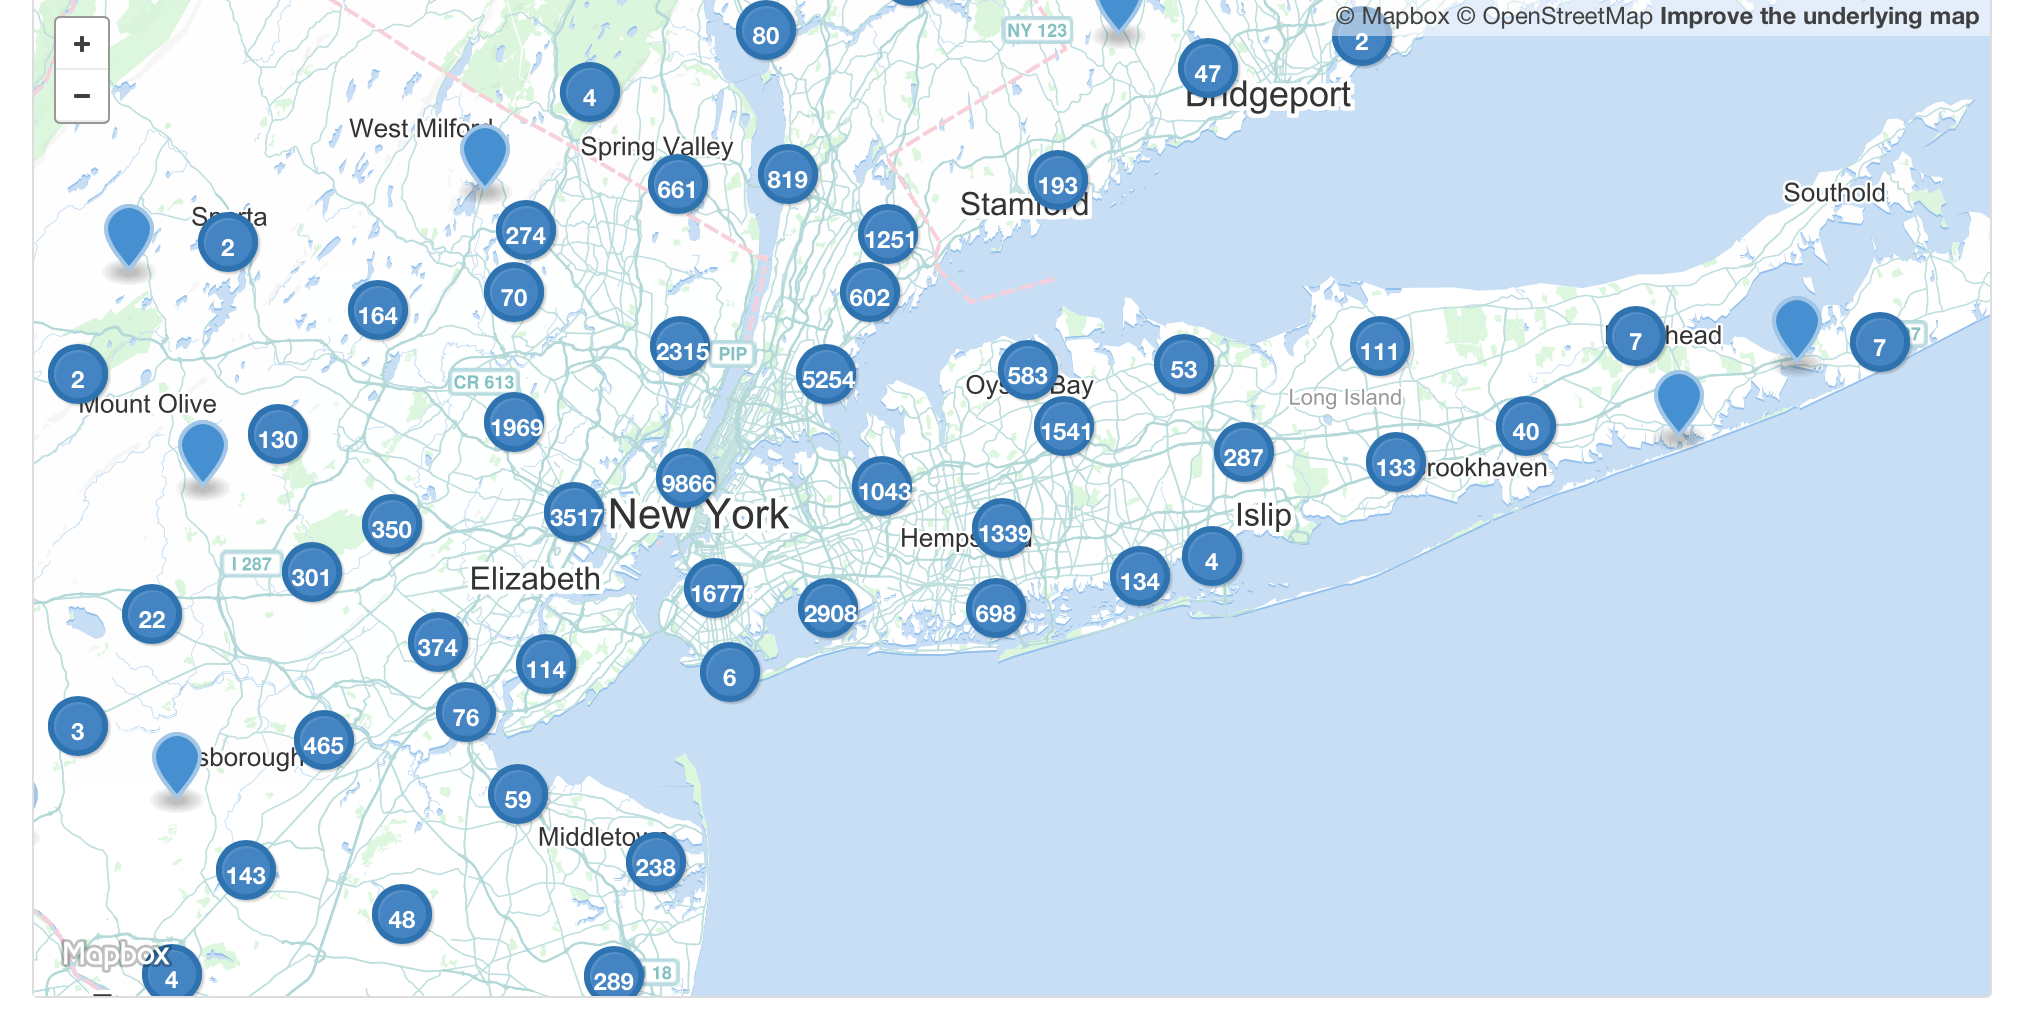
\includegraphics[width=13.3cm, height=7cm]{GeoJson}  \\

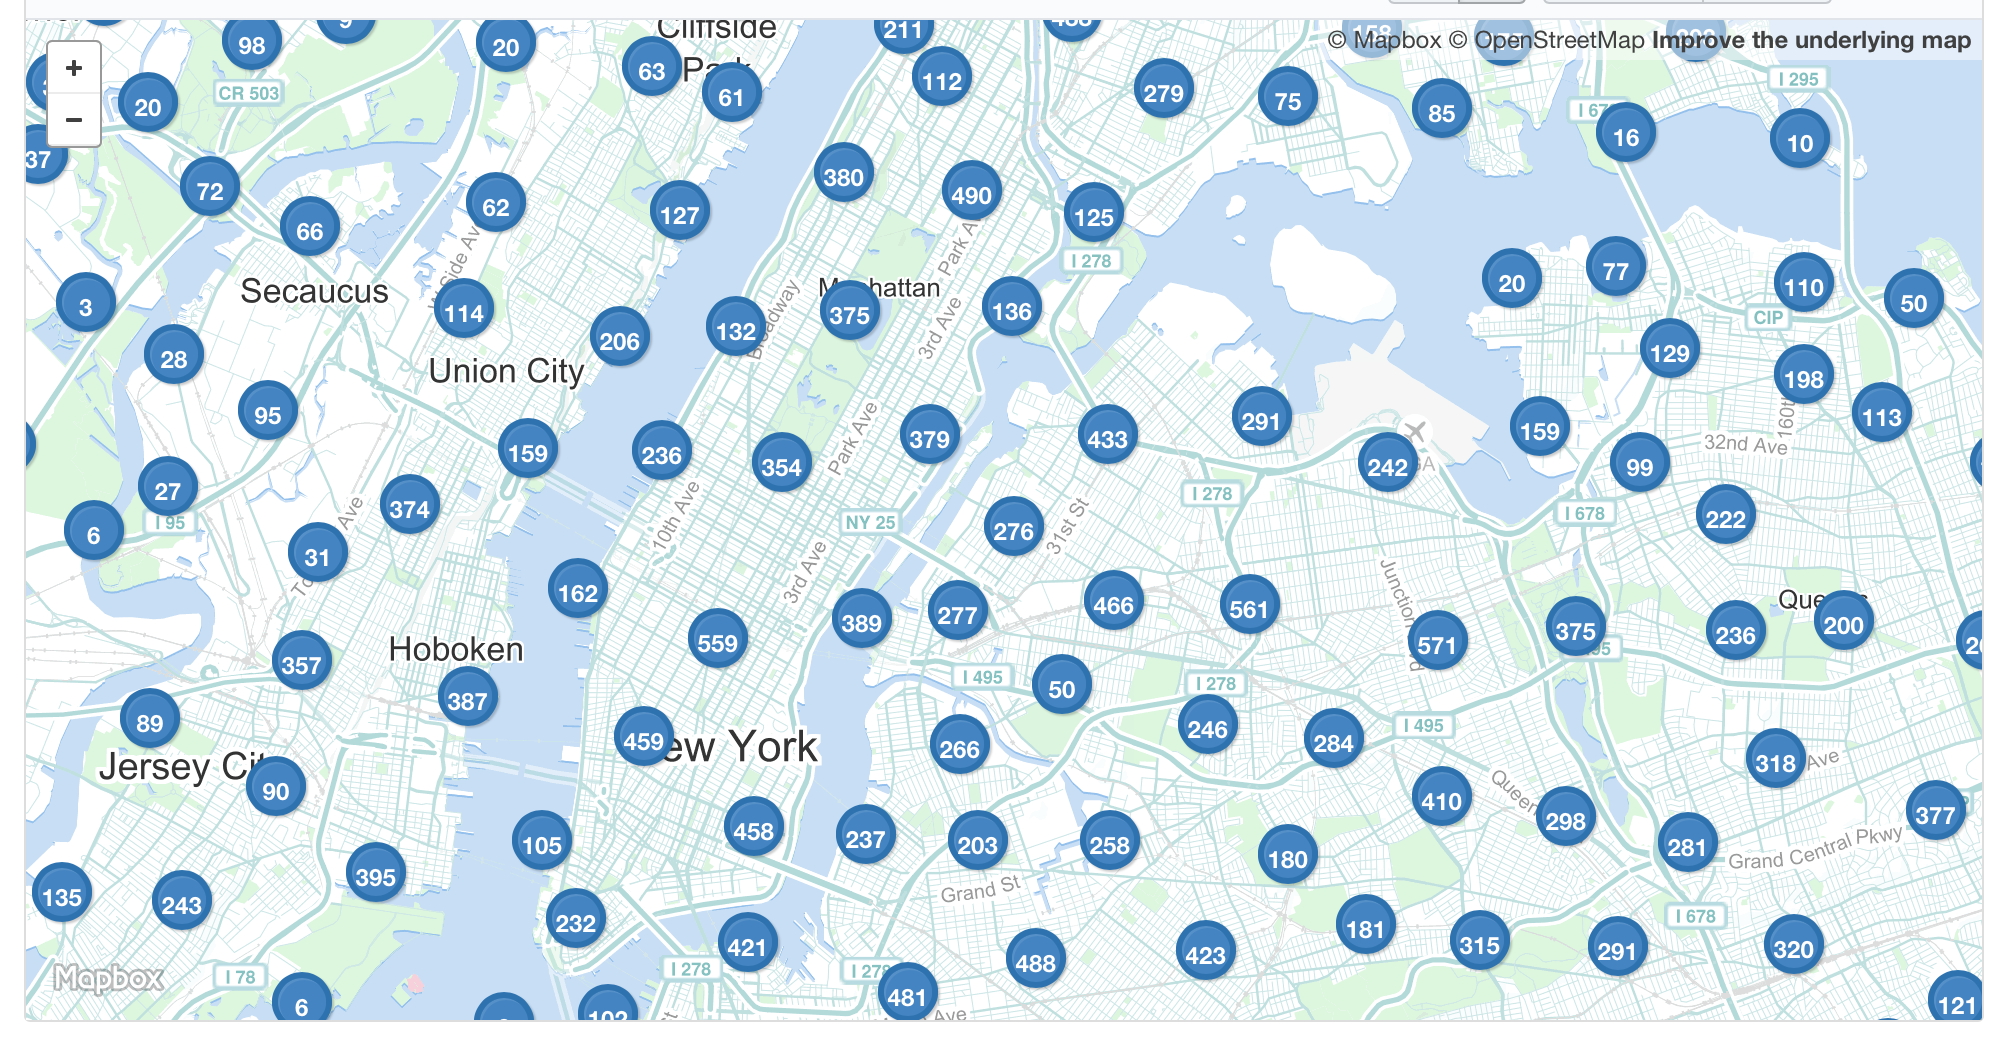
\includegraphics[width=13.3cm, height=7cm]{NewYorkGeoJson} \\


Both of the above images represent the number of uber pickup at different zoom levels. This provides a dynamic view to grid and choose parameters for future analysis.

\break

\paragraph{4 Random Forest Regressor} ~\\
\paragraph{4.1 Introduction} ~\\

In random forests each tree in the ensemble is built from a sample drawn with replacement from the training set. In addition, when splitting a node during the construction of the tree, the split that is chosen is no longer the best split among all features. Instead, the split that is picked is the best split among a random subset of the features. As a result of this randomness, the bias of the forest usually slightly increases but, due to averaging, its variance also decreases, usually more than compensating for the increase in bias, hence yielding an overall better model.

For our dataset the features that we feed to train random forest regressor are binning centers, epoch time stamps with the label as number of pickups. We used 5 months of data as our training data and last month data for valadating the model.

\paragraph{4.2 Pre-processing Step} ~\\

To use our data with Random Forest regressor, we did few steps of pre-processing. 

\begin{itemize}
	\item Grid Binning
	\item Epoch Time Conversion
	\item Binning by Time+Grid
\end{itemize}

\paragraph{4.2.a Grid Binning and why it's better than DBSCAN} ~\\

In Grid binning we divide the entire area of NYC into uniformly spaced two dimensional square grids. We do binning by considering all latitude and longitude pairs lying in a grid and then represent them by co-ordinates of the grid center. We represent the grid by row and column it belongs to.By this approach we can reduce the size of data but still maintain the original variance of the data.
Now we need to find centers to represent the grids. One way to do this to find the mean of all the points in the grid and use that point as the new center. A better approach to solve this issue is to use the two dimensional grid coordinates rather than the geographical centers. This works because grid cooridnates are also equally spaced and uniformly distributed as the original geographical centers. 
Doing so, gave us a clear picture of how NYC looks in grids. Here is the picture on 1000x1000 grids. \\


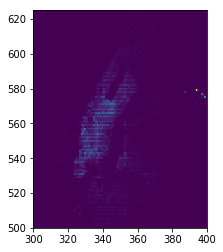
\includegraphics[width=11cm, height=8cm]{binning.png} \\


We can deduce the shape of Manhattan from this HeatMap. We can increase the granularity by increasing the number of grids, but that would outdo the reason why we did binning in the first place.


\paragraph{4.2.b Epoch Time Conversion and why it helps} ~\\

The Unix epoch (or Unix time or POSIX time or Unix timestamp) is the number of seconds that have elapsed since January 1, 1970 (midnight UTC/GMT), not counting leap seconds (in ISO 8601: 1970-01-01T00:00:00Z) 
This convert the standard date-time string to a number, as it acts as one of the input for Random Forest Regressor. \\
\break

\paragraph{4.2.c Binning on Time and Grid} ~\\

We bin on time and grid together and find number of Uber pickups for each unique combination. We use the count as Y label for random forest regressor(estimator). 


\paragraph{4.3 Results} ~\\

Prediction accuracy was 89\% with Random Forest Estimator. We used 5 months starting from April to August as training data and September data as testing data. We used a mean error of 1 ride for finding the accuracy.  \\

Prediction Accuracy =  89\% \\

Root Mean Square Error =  1.7914\\

\break
\paragraph{5 GPFlow} 
\paragraph{5.1 Introduction} ~\\

Gaussian process�is a statistical model where observations occur in a continuous domain. From the results of exploratory analysis we concluded that our data is continuous in time and we can implement Gaussian Process Regression with Periodic Kernels to study the trends in Uber Pickups daily, hourly or weekly. We used GPFlow building Gaussian process models in python, using�TensorFlow.

\paragraph{5.2 Data Pre-Processing} ~\\

We had the data with features like date and time of pickup over 6 months. We transformed the data by binning data by hour i.e we assumed starting date and time of our data to be first hour and then counted Uber pickups by each hour ranging from April 1st  12:00 am to Sep 30th 12:00 pm. This was done so that we can apply and experiment with Periodic Kernels (Hourly, Weekly or Daily) \\

We also scale our features like number of pickups by dividing it by the max number of pickups, this results in value for number of pickups to be scaled down to number between zero and one. We noticed that doing such scaling makes GPFlow faster and we get more accurate metrics out of the library.\\


We take three kernels 
\begin{itemize}
\item km = GPflow.kernels.Matern52(1, lengthscales=12*24.0)
\item k724 = GPflow.kernels.PeriodicKernel(1, period=7*24.0)
\item k24 = GPflow.kernels.PeriodicKernel(1, period=24.0)
\end{itemize}

First Kernel is a Matern5/2 Kernel with a defined length scale (lengthscale�determines the length of the 'wiggles' in your function. In general, you won't be able to extrapolate more than units away from your data). Next kernel is a periodic kernel defined for weekly trends and third kernel covers daily trends. These kernels are experimented with different configurations to maximize the log likelihood.  \\

Optimization is done by calling m.optimize() which has optional arguments that are passed through to�scipy.optimize.minimize�(we minimize the negative log-likelihood).

\paragraph{5.3 Gaussian Process Regression} ~\\

Training data are D = { $x^{i}$  ,$y^{i}$ $\mid$ i = 1, . . . , n}. 

\begin{itemize}
	\item Our training data for Uber is an input vector x of 4 dimensions that is latitude, longitude, date and time. 
	\item Each target is a real valued scalar y = f (x) + noise. Here f(x) is number of pickups for us
	\item Collect inputs in (d x n) matrix in X, and targets in vector, \\ 

	\centerline {Y: D = \{X, Y\} }

	\item We wish to infer f * (number of pickups) for unseen input x * , using P(f * $\mid$  x* , D). So, for any unseen input given coordinates (latitude and longitude), date, time and the training data.


\item This is an (n x d) dimensional feature map $\Phi$  

\begin{center}
$
\Phi = 
\begin{bmatrix}
. & . & \overrightarrow{\phi}(X_{1})^{T} &.  & .  &\\ 
. & . & \overrightarrow{\phi}(X_{2})^{T} &.  & .  &\\ 
. & . & .&. & . & \\ 
. & . & . &.  & .  & \\ 
. & . & \overrightarrow{\phi}(X_{n})^{T} &.  & .  & 
\end{bmatrix}
$ 
\end{center}

\item A Gaussian process is a collection of random variables, any finite number of which have a joint Gaussian distribution. $\Phi$ is (n x d) dimensions and $\phi$ is (1 x d) i.e one row of feature map. K defines joint distribution over function values. Therefore GP specifies a distribution over funtions   

\begin{center}
$K_{nm} = \lambda ^{-1} \left ( \Phi \Phi ^{T} \right )$ \break

$K_{nm}  = \frac{1}{\lambda } \overrightarrow{\phi }\left ( \overrightarrow{X_{n}} \right )^{T}\overrightarrow{\phi }\left ( \overrightarrow{X_{m}} \right ) $ \break

$K_{nm} = \frac{1}{\lambda } l\left [ \overrightarrow{X_{n}},\overrightarrow{X_{m}} \right ]$ \break

\end{center}

\item Here K is our Kernel Matrix $\Phi$  

\begin{center}

$ K := \phi \phi ^{T}$ \break

\end{center}

\item As per Linear Rigression feature map is:: \\

\begin{center}
\(\theta\)   = $(XX^{T})^{-1}X^{T}Y$ 

\end{center}



\item Maximum a Posteriori (Expected Values of Weights) D X D inversion \\

\begin{center}

$E\left [w/y  \right ] =  A^{-1}\phi ^{T}Y$\ 
\tab
$A = (\phi^{T} \phi + \lambda I )$ \break
\end{center}

\item Maximum a Posteriori (Expected Values of Weights) N X N inversion \\
\begin{center}
$K =  \lambda ^{-1} \left ( \Phi \Phi ^{T} \right )$ 
\tab
$A^{-1}\phi ^{T} = \phi ^{T}\left ( K + \lambda I^{-1} \right )$ \break
\end{center}
\item Predictive Posterior using Kernels
\begin{center}


$E\left [ f\left ( x\star  \right ) \mid y \right ] = \phi \left ( x\star  \right )^{T}E\left [ w/y \right ]$ \\

${\mathbb{E}}[\frac{f(x_{\star })}{y}] =  \phi (x_{\star })^{T}{\mathbb{E}}[\frac{w}{y}]$ 

${\mathbb{E}}[\frac{f(x_{\star })}{y}] =  \phi (x_{\star })^{T}\Phi^{T}(K + \lambda I)^{-1}y$

${\mathbb{E}}[\frac{f(x_{\star })}{y}]  = \sum_{n,m}k(x_{*},x_{n})(K + \lambda I)^{-1}_{nm}y_{m}$
\end{center}

\end{itemize}

\break


\paragraph{6 Trends} 

\paragraph{6.1 Trends for April}  ~\\

We apply Gaussian process regression for Uber pickups data of April, the plot of mean, covariance and confidence intervals shown below. In this plot marker 'x' represents the data point. Blue line is mean of the Gaussian that we fit. There is also a light blue fill represents confidence intervals (variance). After optimizing and maximizing the log likelihood the mean of the Gaussian is a good fit.  Another important change was to fix the kernels parameters so that re-running the optimization of GPFlow model does not change the log likelihood values. \\

\begin{center}
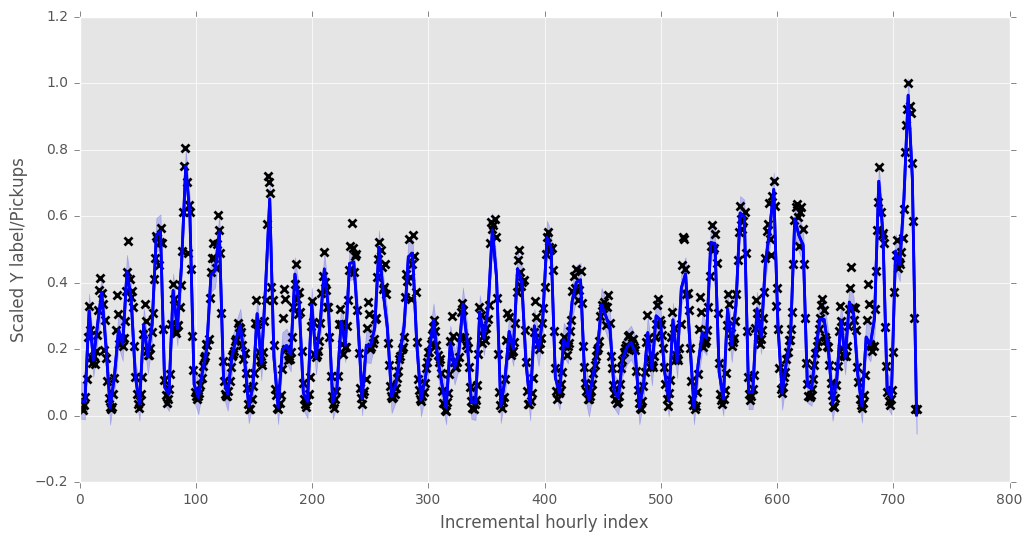
\includegraphics[width=12cm, height=8cm]{April1} 
\end{center}

The image below shows the residual plot that is plotting the data by subtracting the mean of GP model from each data point. Looking at this figure we can conclude that more than 95\% of the data is within 5\% range of the mean we fit. This also gives us a hint to look at points which are substantially away from the mean. So these points are the hours where Uber had substantial increase in its pickups. We need to investigate the reasons for this increase and hence we do the analysis factors like change in temperature, precipitation(rainfall), public holidays (state or federal) or any incident that accounts for this increase in Uber pickups.
\begin{center}
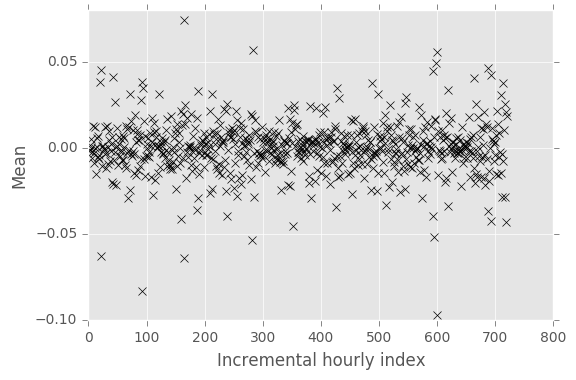
\includegraphics[width=12cm, height=7cm]{April2} 
\end{center}
The image below shows the scaled plot of the mean of Uber Pickups (mean of the Gaussian Model) cumulated by a day, daily change in weather and change in precipitation. We notice one thing consistently, i.e whenever there is precipitation or sharp changes in weather, the Uber pickups substantially increase.We also notice one thing that we see drop in Uber pickups during mid-week.

\begin{center}
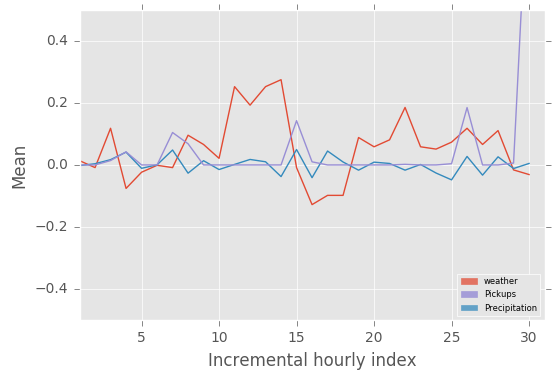
\includegraphics[width=12cm, height=7cm]{April3} 
\end{center}

The table shows a list of points where uber pickup substantially increased as compared to the mean.

\begin{center}
 \begin{tabular}{||c c c||} 
 \hline
 Date & Pickups & Reason\\ [0.5ex] 
 \hline\hline
 2014-04-12 18:00:00 & 1167 & Saturday Night\\ 
 \hline
 2014-04-26 01:00:00 & 1162 & Rainfall\\
 \hline
 2014-04-07 19:00:00 & 2035 & Rainfall\\ [1ex] 
 \hline
\end{tabular}
\end{center}

\paragraph{6.2 Trends for July}  ~\\

The below image shows residual graph for July. We can see that more than 97\% of the data is within 4\% of variance and we get certain points where Uber pickups substantially increased as well as certain points with substantial drop in Uber pickups. We will now analyze these sudden change in Uber pickups on these points in regards with weather or any other activity \\

\begin{center}
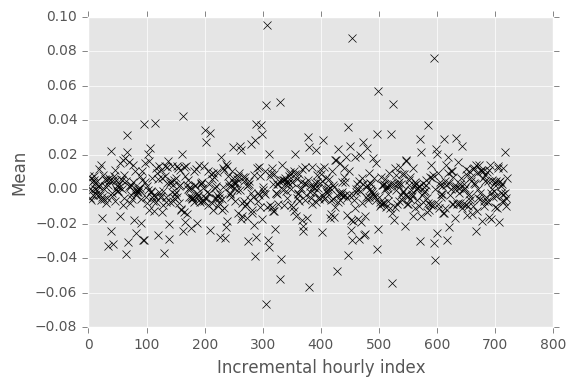
\includegraphics[width=12cm, height=8cm]{June1} 
\end{center}

Scaled plot of temperatures, precipitation and mean of our Gaussian suggests that every time there was rainfall, Uber pickups substantially increased. This trend can be easily verified in regards with other months as well. Also we know that 4th of July is Independence day and we see a sharp decline in Uber pickups on that federal holiday. Some other observations also suggest increase in Uber pickups with increase in temperature.

\begin{center}
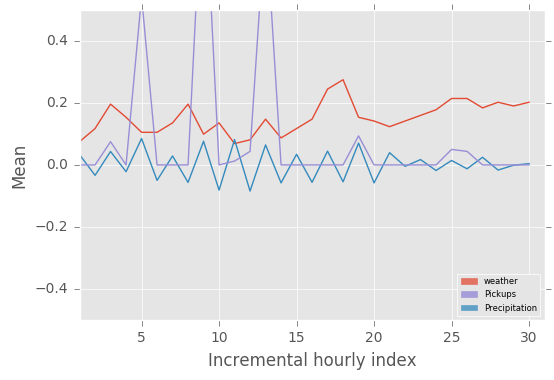
\includegraphics[width=12cm, height=8cm]{June2} 
\end{center}

\paragraph{6.3 Outliers in residual graph for complete dataset}  ~\\

Apart from the general trend we observed due to changes in precipitation or temperature across our dataset, we did observe a few outliers (unexpected increase in number of pickups) which can be attributed to important events (manmade events like games,accidents which don't occur periodically) that have had happened around the pickup location. A few important one are listed below

\begin{itemize}
\item  May 03 2014 [ High pickups ] : Revlon marathon happened on this day which attracted lot of New Yorkers to this event. Also, there was an NYC subway rail accident due to which NYC subway was shut for a few hours.
\item April 13 2014 [ High pickups ] : Baseball match between Boston Red Sox and New York Yankees.
\item May 26 2014, July 4 2014 [ Low pickups ] : Due to memorial day and independence day the number of pickups were low.
\item September 12 2014 [ High pickups ] : Baseball match between Baltimore orioles and New York Yankees.
\item May 24 2014 [ High Pickups ] : March against Monsanto NYC at Union Square.
\item June 13 2014 [ High Pickups ] : Baseball match between San Diego Padres vs New York Mets.
\end{itemize}

\paragraph{6.4 Weekend Vs Weekday Trend} ~\\

The plot on the left represents the uber pickup during the Mondays and the right shows pickups during Fridays night, we can clearly identity the area where most of the commercial buildings are situated (5,6,7,Madison,Park Ave).\\


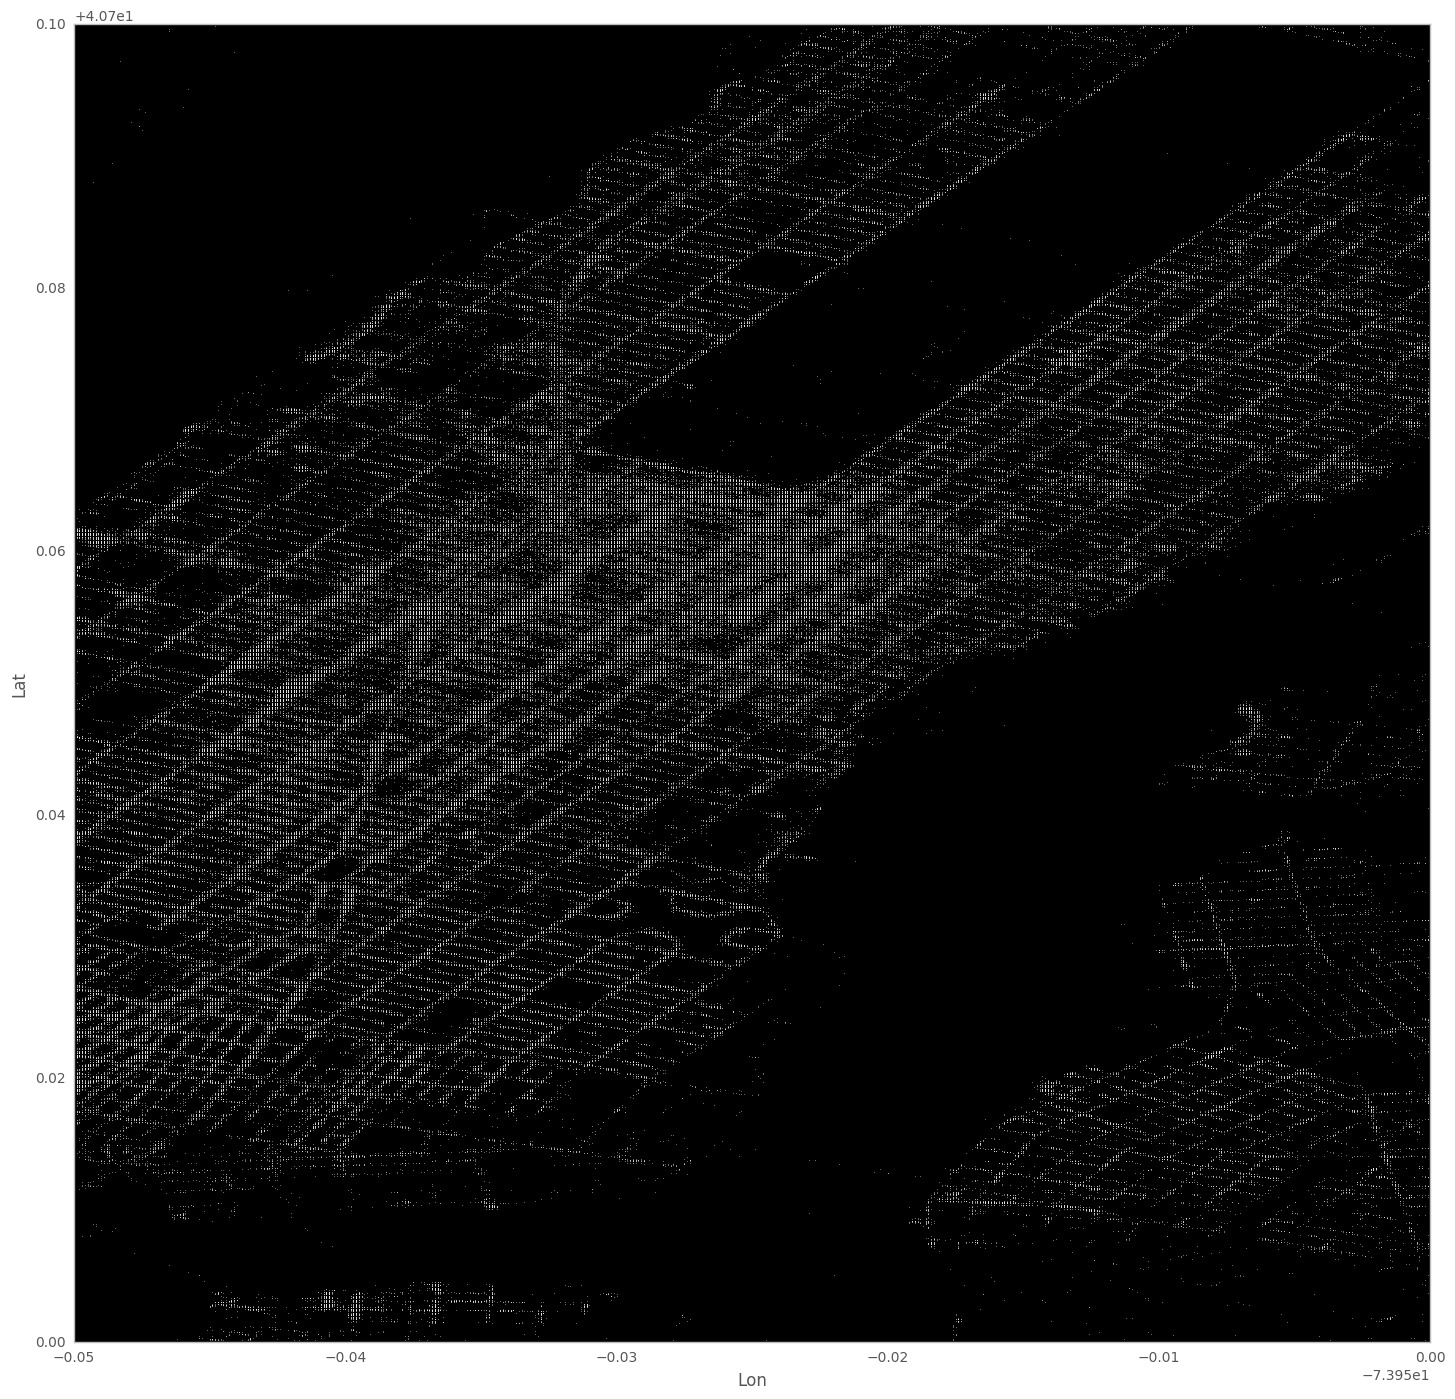
\includegraphics[width=6cm, height=8cm]{monday} 
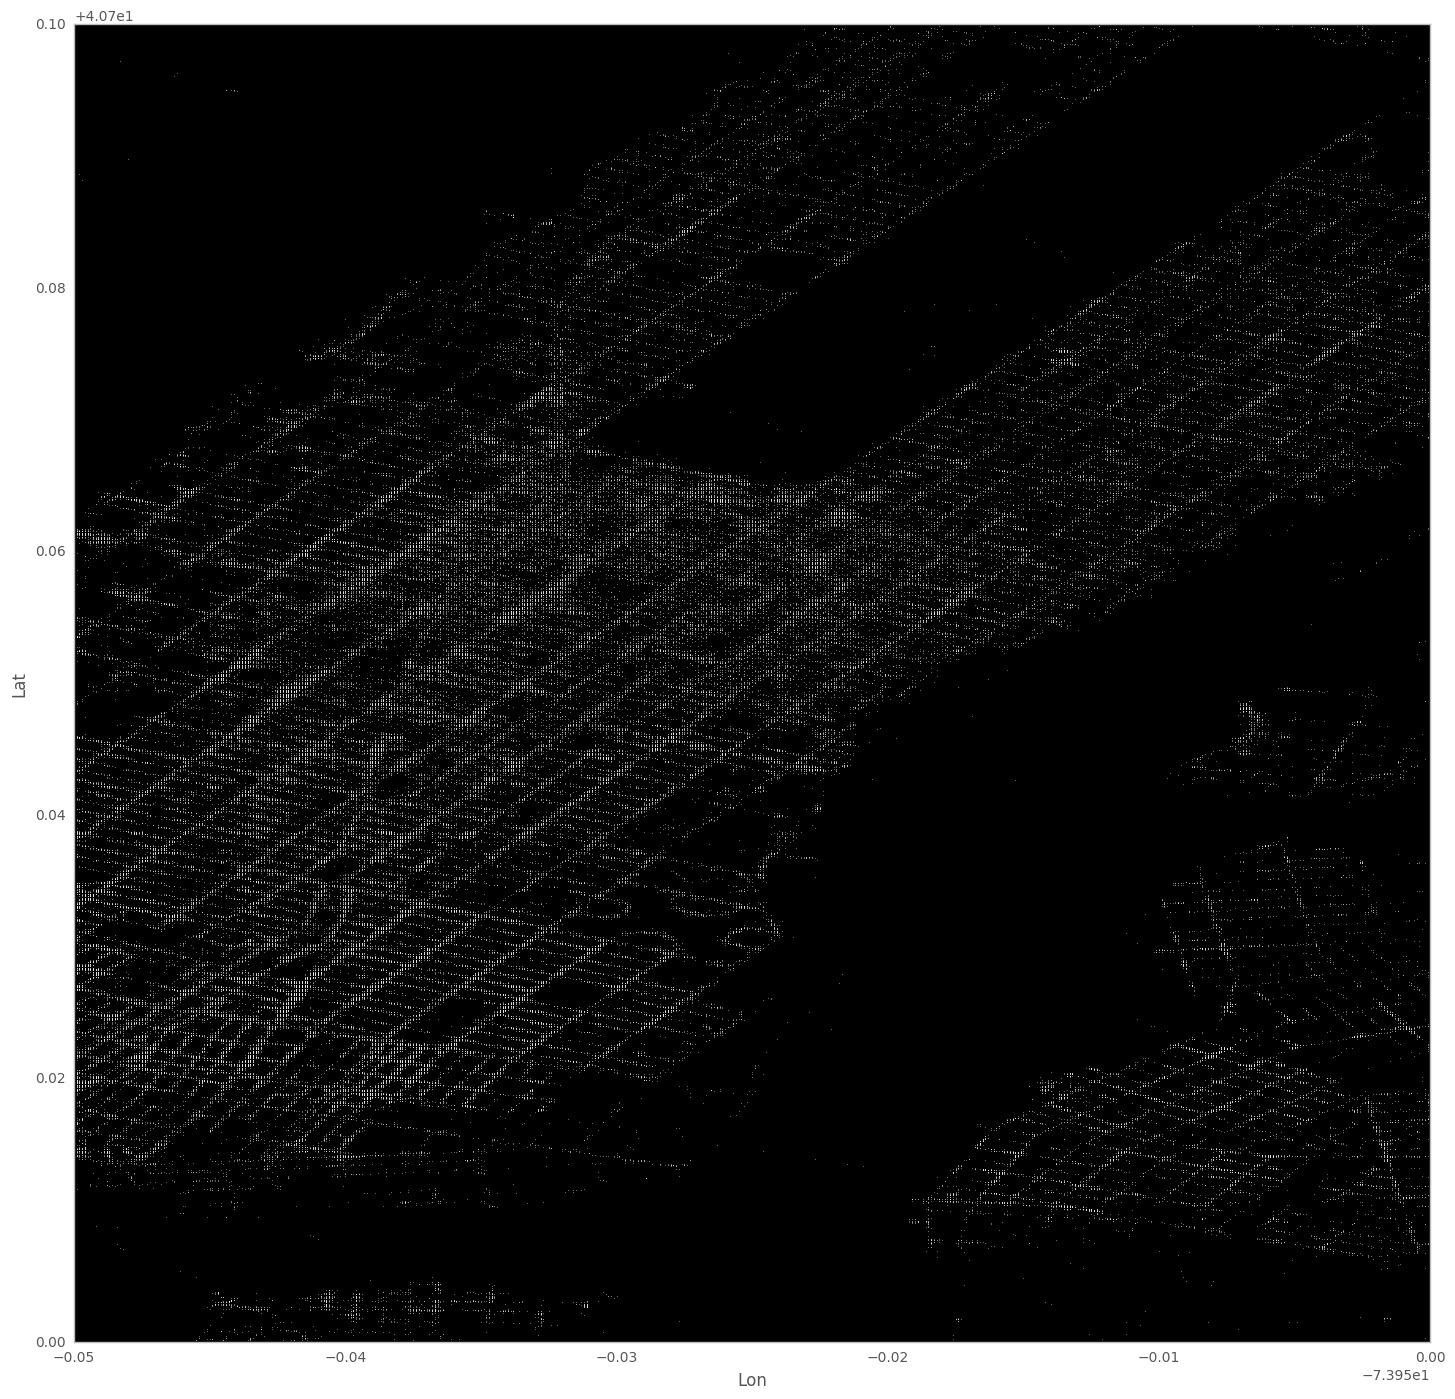
\includegraphics[width=6cm, height=8cm]{friday}


\break

\paragraph{7 Conclusions} ~\\

Goal of the project was to predict the number of pickups given the location and time, analyze the pickup trends across the month,day and weeks, study the change in uber pickup with change in temperature and precipitation and also investigate other possible reasons. The purpose behind our goal can potentially help uber to stage more drivers in the areas that could possible have more pickups and reduce the waiting time for their customers.\\

We did exploratory analysis to understand the dense areas by visualizing the distribution of pickup points, the rate of change of number of pickups by hour/day/week/month. Our exploratory analysis included histograms, density plot using choropleth and GeoJSON plotting. By these, we established that our data was continuous and we also removed the noise points. \\

We achieved  89\% accuracy and RMSE of 1.791 with Random forest regressor to predict number of Uber pickup given location and time. \\

GPFlow regression helped us determine the trends in our dataset as a function of time. By toggling our periodic and mattern kernel, we were able to conclude that the data points were directly affected by precipitation, weather and also the outliers caused due to random important events in New York city. We saw an increase in pickups whenever there was rain or any important events like a baseball match, while there were decrease in pickups on Federal holidays.

\paragraph{8 Source Code:} 
\begin{itemize}
\item \href{https://github.com/msabhi/mining-uber-dataset}{Source Code}
\end{itemize}

\paragraph{9 References:} ~\\
\begin{itemize}
\item \href{https://www.linkedin.com/pulse/amazing-ways-uber-using-big-data-analytics-bernard-marr}{https://www.linkedin.com/pulse/amazing-ways-uber-using-big-data-analytics-bernard-marr}
\item \href{http://geojson.org/}{http://geojson.org/}
\item \href{https://github.com/GPflow/GPflow}{https://github.com/GPflow/GPflow}
\item \href{http://stackoverflow.com/}{http://stackoverflow.com/}
\item \href{http://toddwschneider.com/posts/analyzing-1-1-billion-nyc-taxi-and-uber-trips-with-a-vengeance/}{http://toddwschneider.com/posts/analyzing-1-1-billion-nyc-taxi-and-uber-trips-with-a-vengeance/}
\item \href{https://www.ncdc.noaa.gov/}{https://www.ncdc.noaa.gov/}
\end{itemize}
\end{document}